
\begin{figure}[H]
  \centering
  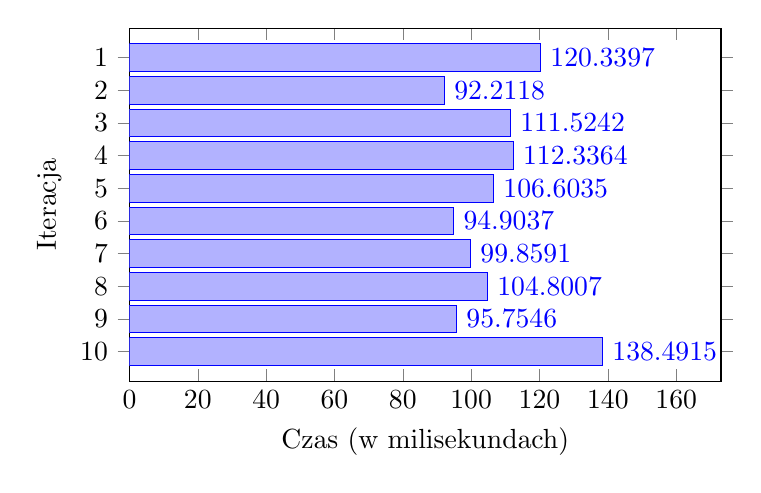
\begin{tikzpicture}
  
    \begin{axis} [
      xbar = .05cm,
      nodes near coords,
      nodes near coords style={
        /pgf/number format/precision=4,
      },
      xmin = 0,
      ytick = data,
      enlarge x limits = {value = .25, upper},
      symbolic y coords = {10,9,8,7,6,5,4,3,2,1},
      xlabel=Czas (w milisekundach),
      ylabel=Iteracja,
      width=0.75\textwidth,
      height=0.5\textwidth
    ]
    
      \addplot coordinates {(120.3396999835968,1) (92.21180003881454,2) (111.52419996261597,3) (112.33640003204346,4) (106.60350000858307,5) (94.90369999408722,6) (99.859099984169,7) (104.80070000886917,8) (95.75459998846054,9) (138.49149996042252,10)};
      
    \end{axis}
  
  \end{tikzpicture}
  \caption{Wynik testów przykładu 2 [\ref{lst:wydajnosc-przyklad-p-2}]}
  \label{fig:wynik-przyklad-1}
\end{figure}
